\documentclass{article}
\usepackage[utf8]{inputenc}
\usepackage{enumitem}
\usepackage{listings}
\usepackage{amsmath,amssymb}
\usepackage{geometry}
\usepackage[T1]{fontenc}
\usepackage{graphicx}


\geometry{
 a4paper,
 left=38mm,
 right=38mm,
 top=38mm,
 bottom=38mm
 }

\lstset{
    language=C,
    showstringspaces=false,
    breaklines=true
}



\title{ME 333 Homework 7}
\author{Marshall Johnson}
\date{February 22, 2022}

\begin{document}

\maketitle

\section*{Chapter 24: Feedback Control of LED Brightness}

\setcounter{section}{24}
\setcounter{subsection}{4}
\subsection{Plotting Data in Python}
The following chart was generated using matplotlib in Python. \\

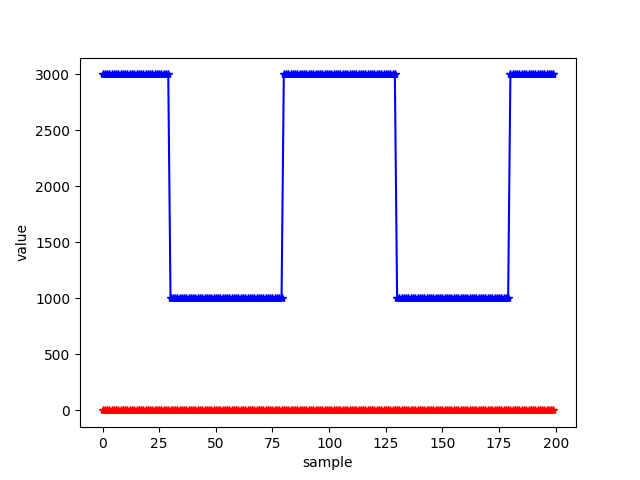
\includegraphics[width=\linewidth]{matplotlib.png}

\pagebreak
\setcounter{subsection}{6}
\subsection{Reading the ADC}
Chart showing REFArray (blue) and ADCArray (red): \\

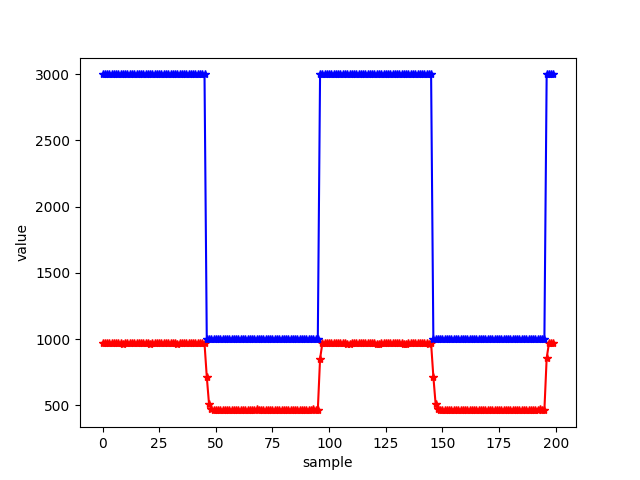
\includegraphics[width=\linewidth]{reading_the_adc.png}

\subsection{PI Control}
Plot of PI controller performance using $K_i = 0.007$ and $K_p = 0.05$:

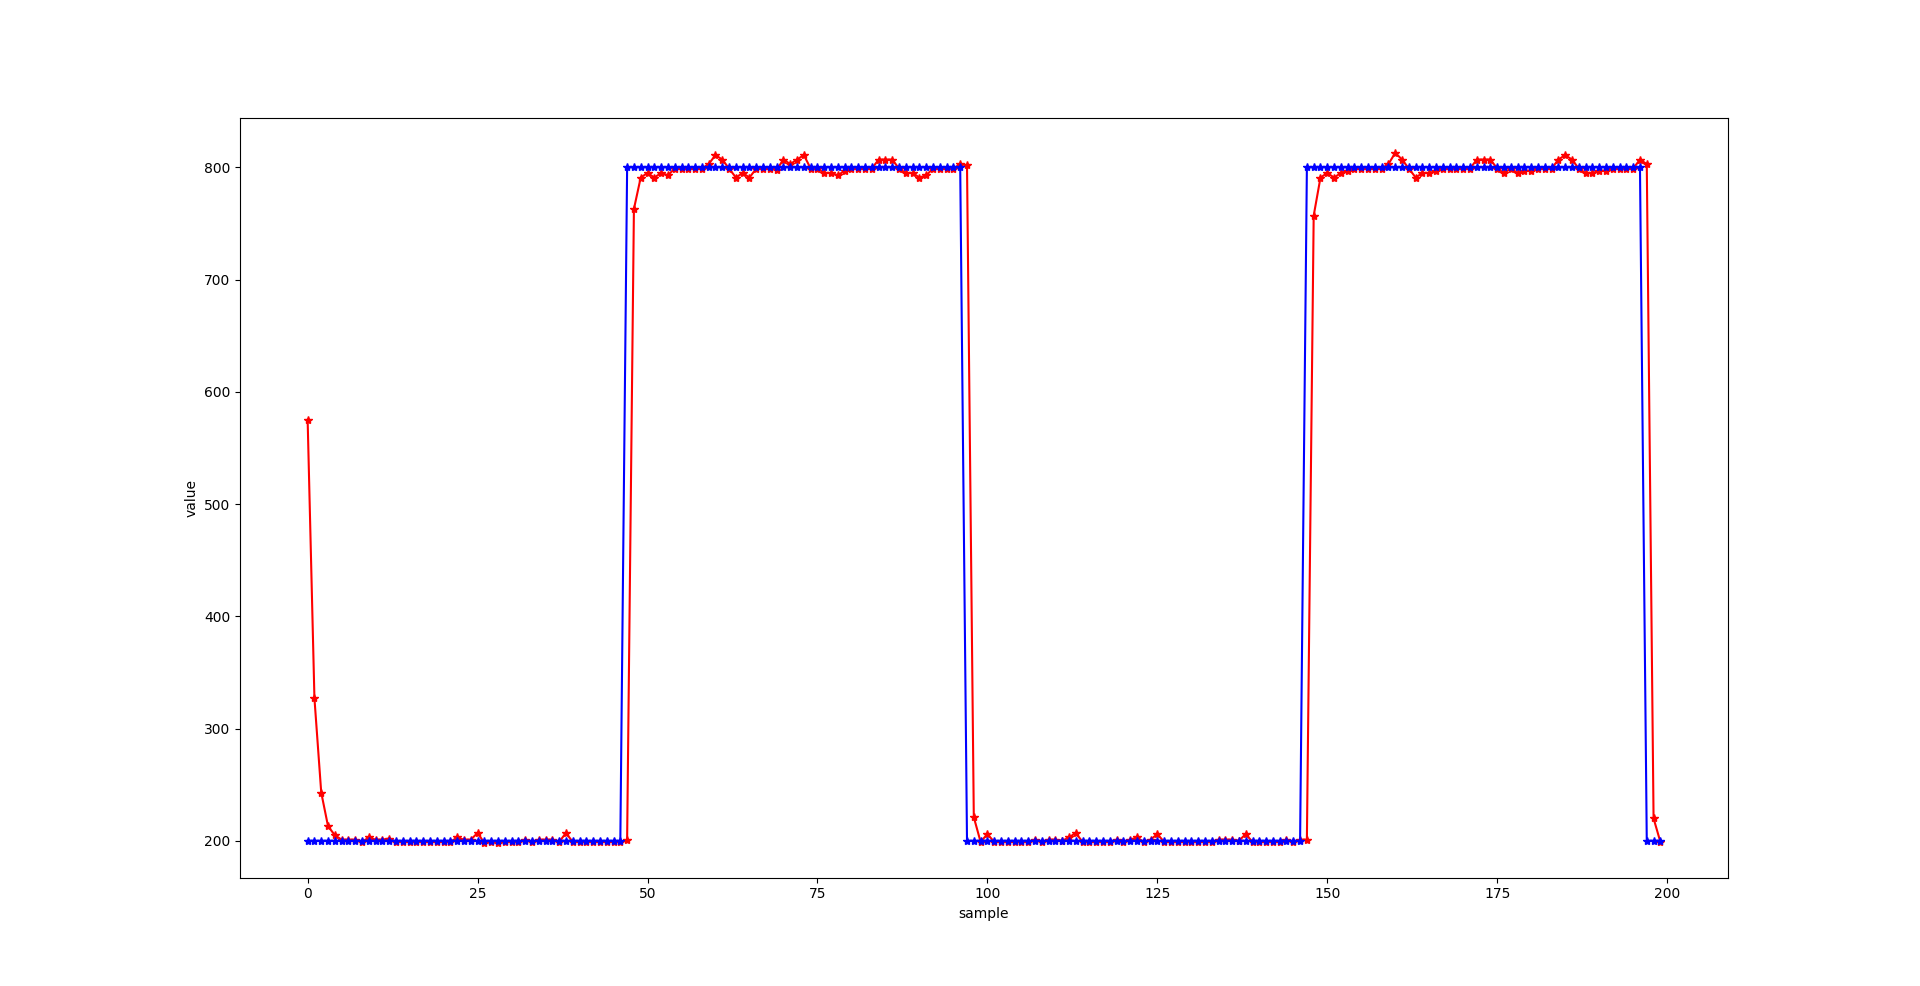
\includegraphics[width=\linewidth]{pi_control_final.png}
See good\_gains.mov for demonstration using the gains above. 
For a demonstration using bad gains, see bad\_gains.mov.

\end{document}
